\documentclass[11pt,a4paper]{article}

\usepackage[margin=2.35cm]{geometry}
\usepackage[T1]{fontenc}
\usepackage[utf8]{inputenc}
\usepackage[english]{babel}
\usepackage{lmodern}
\usepackage{microtype}
\usepackage{amsmath,amssymb}
\usepackage{booktabs}
\usepackage{graphicx}
\usepackage{longtable}
\usepackage{tabularx}
\usepackage{array}
\usepackage{enumitem}
\usepackage{xcolor}
\usepackage{hyperref}
\usepackage{fancyhdr}
\usepackage{listings}

\definecolor{hhublue}{RGB}{0,70,127}
\definecolor{lightblue}{RGB}{235,244,250}
\definecolor{codegray}{RGB}{246,247,248}

\hypersetup{
  colorlinks=true,
  linkcolor=hhublue,
  urlcolor=hhublue,
  pdftitle={NanoGPT Slowrun Seminar Concept Notes},
  pdfauthor={Ahmed Moustafa}
}

\pagestyle{fancy}
\fancyhf{}
\lhead{NanoGPT Slowrun Ablation Study}
\rhead{Seminar Notes}
\cfoot{\thepage}
\renewcommand{\headrulewidth}{0.4pt}

\setlist[itemize]{leftmargin=1.6em,itemsep=0.25em,topsep=0.35em}
\setlist[enumerate]{leftmargin=1.8em,itemsep=0.25em,topsep=0.35em}
\setlength{\parindent}{0pt}
\setlength{\parskip}{0.55em}
\renewcommand{\arraystretch}{1.18}

\lstset{
  basicstyle=\ttfamily\small,
  backgroundcolor=\color{codegray},
  frame=single,
  rulecolor=\color{gray!35},
  columns=fullflexible,
  keepspaces=true,
  showstringspaces=false,
  xleftmargin=0.4em,
  xrightmargin=0.4em,
  aboveskip=0.55em,
  belowskip=0.55em
}

\newcommand{\keypoint}[1]{%
  \begin{center}
    \fcolorbox{hhublue}{lightblue}{%
      \parbox{0.91\linewidth}{\textbf{Key point.} #1}%
    }
  \end{center}
}

\title{\textcolor{hhublue}{NanoGPT Slowrun Seminar Notes}\\
  \large Model Architecture, Evaluation, and Weight Averaging}
\author{Ahmed Moustafa}
\date{Deep Learning Seminar, Summer Semester 2026}

\begin{document}

\maketitle
\thispagestyle{fancy}

\begin{abstract}
These notes explain the overall GPT data flow, the detailed Slowrun architecture,
the components ablated in the presentation, the validation-loss calculation, and
the raw, exponential-moving-average (EMA), and checkpoint-averaged models. The
notation matches the presentation and the repository implementation.
\end{abstract}

\tableofcontents

\clearpage
\section{The Overall GPT Model}

A GPT model is an autoregressive sequence model: it reads the tokens available
so far and predicts the next token. The same network is applied at every token
position, but a causal mask prevents a position from seeing future tokens.

The complete data flow is

\begin{equation}
  \begin{aligned}
    \text{token IDs}
    &\longrightarrow \text{token representations}
    \longrightarrow \text{Transformer blocks}\\
    &\longrightarrow \text{vocabulary logits}
    \longrightarrow \text{next-token probabilities}.
  \end{aligned}
\end{equation}

\subsection{Step 1: Token IDs}

Text is first converted into integer token IDs. For example, a tokenizer might
represent

\begin{lstlisting}
Text:      The cat sleeps
Token IDs: [101, 2003, 1037]
\end{lstlisting}

The numbers themselves have no semantic meaning. They are addresses into a
learned embedding table.

\subsection{Step 2: Token Embeddings and Initial Normalization}

For token ID $t_i$, the embedding lookup returns a vector

\begin{equation}
  e_i=E[t_i]\in\mathbb{R}^{d_{\mathrm{model}}}.
\end{equation}

The vectors are normalized to form the initial hidden representation

\begin{equation}
  x_{0,i}=\operatorname{RMSNorm}(e_i).
\end{equation}

The representation is not a probability distribution. It is a learned feature
vector. Some directions may encode token identity, syntax, topic, or other
features learned during training.

\textbf{Simple example.} The vectors for ``cat'' and ``dog'' may be closer than
the vectors for ``cat'' and ``therefore'' because the model learns that the
first two tokens appear in similar contexts.

This model does not add a learned positional embedding. Position is introduced
inside attention through rotary positional embeddings (RoPE).

\subsection{Step 3: One Transformer Block}

Each block contains two main sublayers: causal self-attention and a SwiGLU MLP.
Both use pre-normalization and a residual connection. A simplified block is

\begin{align}
  a_\ell &= \operatorname{Attention}_\ell
    (\operatorname{RMSNorm}(x_\ell)),\\
  h_\ell &= x_\ell+a_\ell,\\
  m_\ell &= \operatorname{SwiGLU}_\ell
    (\operatorname{RMSNorm}(h_\ell)),\\
  x_{\ell+1} &= h_\ell+m_\ell.
\end{align}

\paragraph{RMSNorm.}
RMSNorm controls the scale of the representation before attention or the MLP.
It does not mix information between token positions.

\paragraph{Causal self-attention.}
Attention lets each token position collect information from permitted earlier
positions. For the sequence

\begin{lstlisting}
[The, cat, sleeps]
\end{lstlisting}

the representation at ``cat'' may use information from ``The'' and ``cat,'' but
not from ``sleeps.'' The representation at ``sleeps'' may use all three tokens.

\paragraph{First residual connection.}
The attention output is added to the previous representation. The model can
therefore preserve the old features and add only the contextual correction it
needs.

\paragraph{SwiGLU MLP.}
The MLP transforms each token position independently after attention has mixed
context across positions. A simplified form is

\begin{equation}
  \operatorname{SwiGLU}(x)
  =W_o\left(\operatorname{SiLU}(W_gx)\odot W_fx\right).
\end{equation}

Attention answers ``which earlier tokens matter?'' The MLP answers ``how should
the collected features be transformed?''

\paragraph{Second residual connection.}
The MLP output is added back to the residual stream. This preserves a direct
information path through many layers.

\subsection{Step 4: Repeating the Blocks}

The laptop model repeats the block four times; the H100 model repeats it 16
times. Early layers commonly learn local or surface-level patterns, while later
layers can combine them into more task-specific predictions.

\textbf{Simple example.}

\begin{itemize}
  \item An early layer may identify that ``cat'' is a noun.
  \item A middle layer may combine ``The cat'' into a subject phrase.
  \item A later layer may use that phrase to increase the logits of plausible
        verbs such as ``sleeps,'' ``runs,'' or ``sits.''
\end{itemize}

These are useful intuitions, not fixed hand-programmed roles. The network learns
its own distributed features.

\subsection{Step 5: From Hidden States to Token Probabilities}

After the last block, the model applies final RMSNorm and a vocabulary
projection:

\begin{align}
  u_i &= \operatorname{RMSNorm}(x_{L,i}),\\
  z_i &= W_{\mathrm{vocab}}u_i.
\end{align}

The logits are soft-capped:

\begin{equation}
  \widetilde z_i=15\tanh(z_i/15).
\end{equation}

The soft-cap limits extremely large logit magnitudes. During inference, softmax
converts logits into probabilities:

\begin{equation}
  p(t_{i+1}=v\mid t_{\le i})
  =\frac{\exp(\widetilde z_{i,v})}
         {\sum_{u\in V}\exp(\widetilde z_{i,u})}.
\end{equation}

If the context is ``The cat,'' a possible distribution is

\begin{lstlisting}
sleeps: 0.60
runs:   0.20
blue:   0.01
other:  0.19
\end{lstlisting}

Training compares this distribution with the correct next token. Softmax is
shown explicitly for inference; the cross-entropy implementation can operate
directly on logits for numerical stability.

\subsection*{Overall GPT Diagram}
\begin{center}
  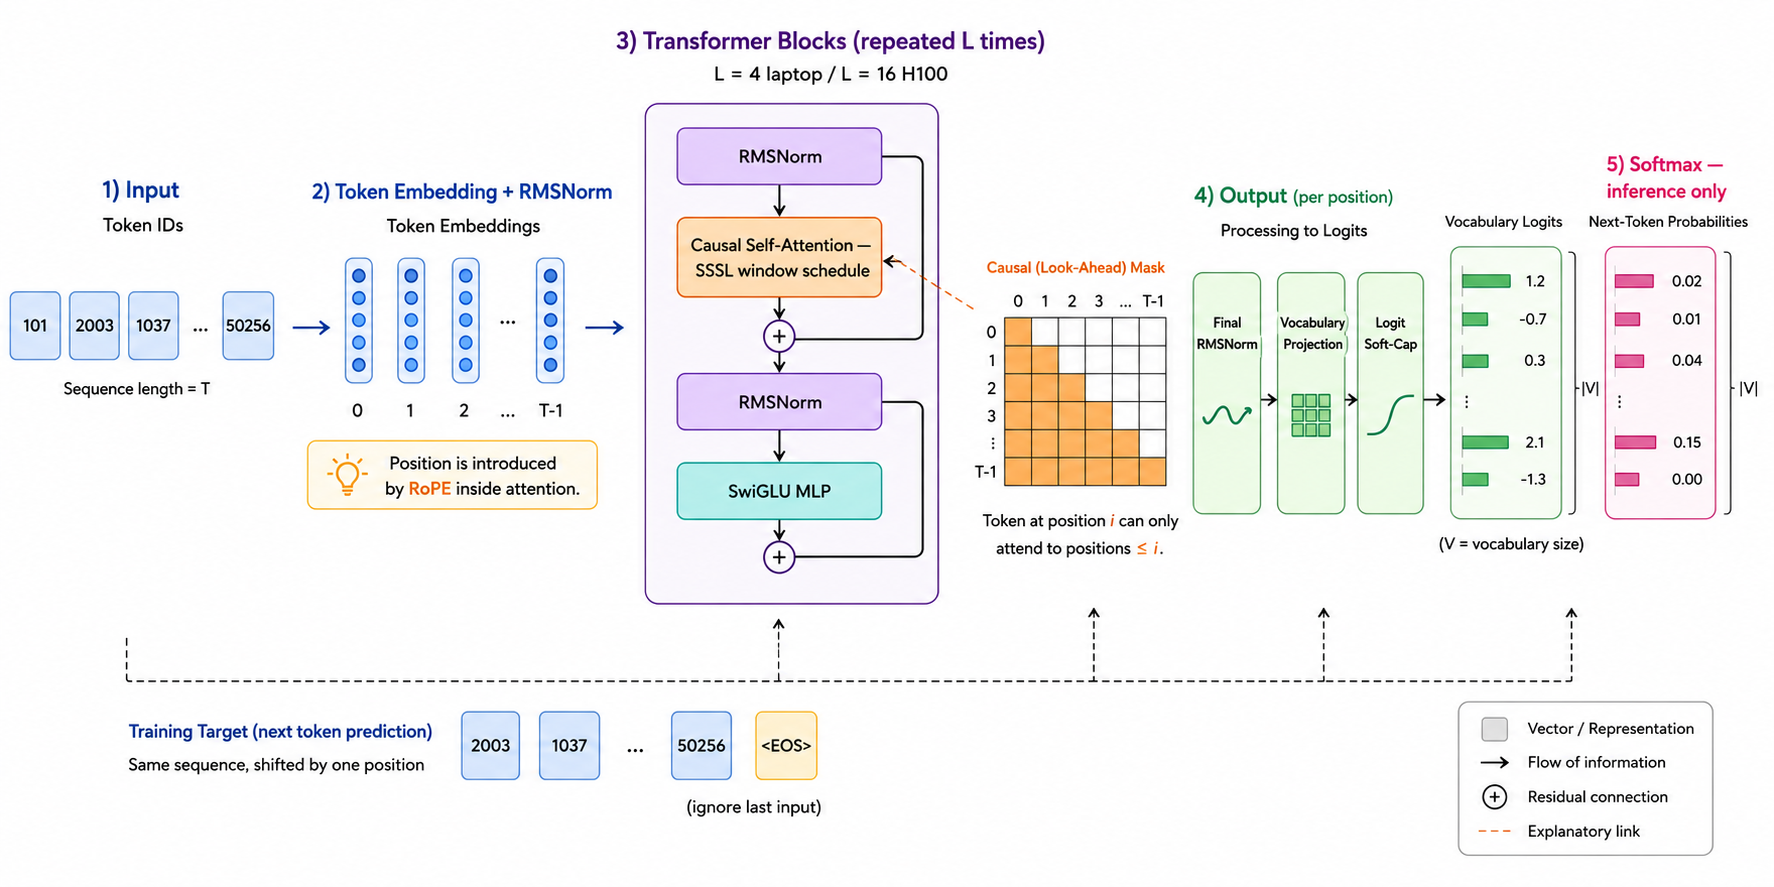
\includegraphics[width=0.94\linewidth,height=0.38\textheight,keepaspectratio]
    {../figures/gpt-simple.png}

  \small Read from left to right: token IDs, normalized embeddings, repeated
  Transformer blocks, vocabulary logits, and inference probabilities. The
  dashed lower path shows the one-token-shifted training target.
\end{center}

\clearpage
\section{The Detailed NanoGPT Slowrun Architecture}

The detailed diagram expands the simplified Transformer block and adds the
Slowrun-specific information paths. Read the central stack from bottom to top.
The separate panel on the right expands the attention sublayer. The arrow colors
have fixed meanings:

\begin{itemize}
  \item \textbf{black:} standard residual paths inside a block;
  \item \textbf{blue:} mirrored U-Net skip connections between layers;
  \item \textbf{green:} value residuals derived from the initial embedding $x_0$.
\end{itemize}

\subsection*{Detailed Slowrun Diagram}
\begin{center}
  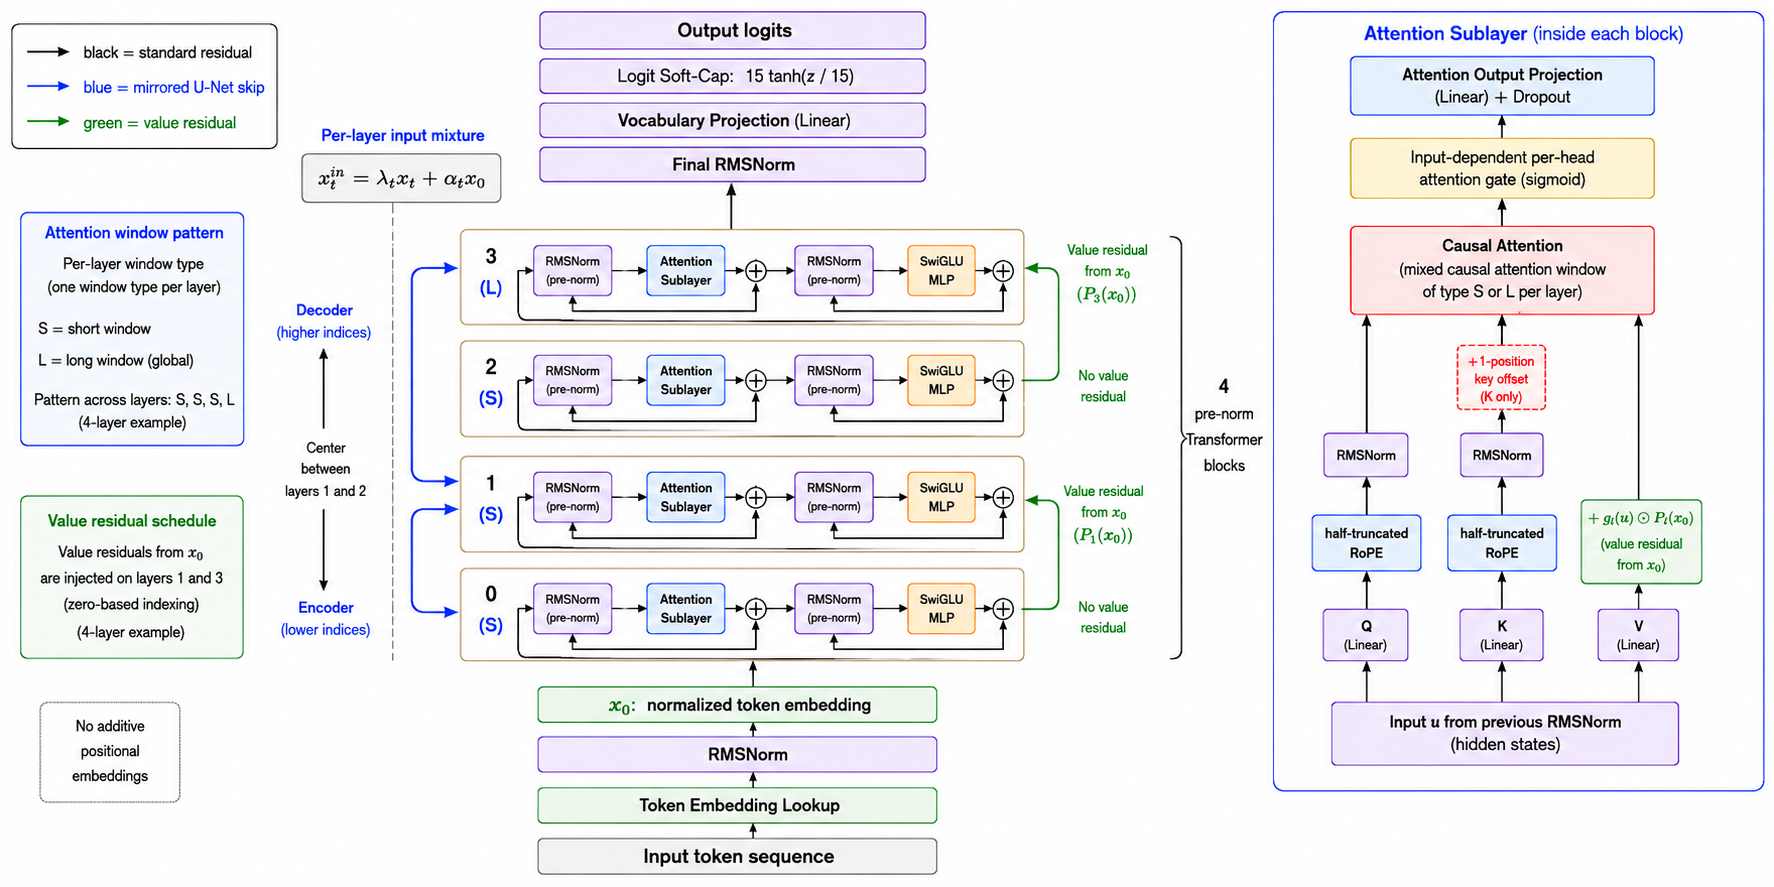
\includegraphics[width=0.96\linewidth,height=0.41\textheight,keepaspectratio]
    {../figures/gpt-detailed.png}

  \small Use the center for the full layer stack, the left callouts for schedules,
  and the right panel for $Q/K/V$, RoPE, key offset, causal attention, and the
  per-head gate.
\end{center}

\subsection{Detailed Data Flow Through One Layer}

At layer $\ell$, the residual stream is first mixed with the initial normalized
embedding:

\begin{equation}
  x_\ell^{\mathrm{in}}
  =\lambda_\ell x_\ell+\alpha_\ell x_0.
\end{equation}

This gives every layer a learned choice between the current deep representation
and the original token-level representation.

\textbf{Example.} Suppose repeated transformations weaken the feature that the
current token is ``cat.'' A positive $\alpha_\ell$ can restore some of the
original token information before the layer processes it.

The pre-attention hidden state $u$ is then normalized and projected into query,
key, and value vectors:

\begin{equation}
  Q=uW^Q,\qquad K=uW^K,\qquad V=uW^V.
\end{equation}

After RoPE, key offset, value residual injection, and causal masking, attention
computes

\begin{equation}
  Y=\operatorname{softmax}\left(
    \frac{QK^\top}{\sqrt{d_h}}+M_{\mathrm{causal}}
  \right)V.
\end{equation}

The per-head gate scales the attention output. The output projection and dropout
map the concatenated heads back to model dimension. A residual connection adds
the result to the layer input. A second RMSNorm, SwiGLU MLP, and residual
connection complete the block.

\subsection{SSSL Attention Windows}

\textbf{Where to look.} See the blue ``Attention window pattern'' callout on the
left and the $S$ or $L$ label beside each central block.

The four-layer pattern is

\begin{equation}
  S,\ S,\ S,\ L,
\end{equation}

where $S$ denotes a short causal window and $L$ a long or global causal window.
The pattern repeats in the deeper model.

\textbf{Effect on the layer output.} Short-window layers emphasize nearby
context and reduce attention cost. Long-window layers can retrieve information
from much earlier tokens.

\textbf{Example.} In ``The cat that chased the mouse finally slept,'' a short
window can model ``finally slept,'' while a long-window layer can connect
``slept'' back to ``cat.''

\section{Slide 22 Architecture Components}

This section corresponds directly to the ``Architecture Changes'' slide. Each
component below states where it appears in the detailed diagram, its formula,
and how changing it affects a layer output.

\subsection{Attention Gate}

\textbf{Where to look.} In the right attention panel, find
``Input-dependent per-head attention gate (sigmoid),'' directly above causal
attention and below the attention output projection.

For attention head $h$, the baseline output is

\begin{equation}
  y_h'=\sigma(a_h(u))\,y_h.
\end{equation}

The strong-gate variant is

\begin{equation}
  y_h'=2\sigma(a_h(u))\,y_h,
\end{equation}

and the no-gate ablation is simply $y_h'=y_h$.

\textbf{Effect on the layer output.} The gate decides how much each attention
head contributes before the heads are concatenated and projected. The baseline
range is approximately $0$ to $1$; the strong variant can amplify a head up to
approximately $2$.

\textbf{Numerical example.} If a head produces

\begin{equation}
  y_h=[0.4,-0.2]
\end{equation}

and its sigmoid gate is $0.5$, the baseline contribution is
$[0.2,-0.1]$. A strong gate with the same pre-activation produces multiplier
$1.0$ and contribution $[0.4,-0.2]$. Removing the gate also gives the unscaled
head output.

\subsection{Mirrored U-Net Skip Connections}

\textbf{Where to look.} In the center stack, follow the blue curved arrows from
lower-index encoder layers to mirrored higher-index decoder layers. In the
four-layer example, layer 0 connects toward layer 3 and layer 1 toward layer 2.

The decoder input includes

\begin{equation}
  x_\ell\leftarrow x_\ell+s_\ell x_{L-1-\ell},
\end{equation}

where $s_\ell$ is a learned skip weight. The no-skip ablation removes the second
term.

\textbf{Effect on the layer output.} The decoder receives an earlier, less
processed representation directly. This can preserve local information and
provide a shorter gradient path.

\textbf{Example.} An early layer may preserve that ``cat'' is the exact input
token, while later layers focus on sentence meaning. The skip lets a later layer
combine both representations without reconstructing the token identity from
scratch.

\subsection{Value Residuals}

\textbf{Where to look.} Follow the green arrows from $x_0$ into alternating
layers in the center stack. In the right attention panel, find the green box
added to the $V$ branch.

The baseline value branch is

\begin{equation}
  \widetilde V_\ell
  =X_\ell W_\ell^V
   +2\sigma(g_\ell(X_\ell))\odot P_\ell(x_0).
\end{equation}

Without the value residual,

\begin{equation}
  \widetilde V_\ell=X_\ell W_\ell^V.
\end{equation}

\textbf{Effect on the layer output.} Attention weights still decide which token
positions to read, but the content retrieved from those positions now contains
a gated projection of the original token representation. The mechanism changes
the values being aggregated, not the attention mask.

\textbf{Example.} Suppose a later layer attends strongly to the earlier token
``cat.'' Its local value vector may mainly encode the grammatical role
``subject.'' The value residual can additionally supply token-identity features
from $x_0$, allowing the output to preserve both ``subject'' and ``cat.''

This was the most important architecture ablation in the small model: removing
it caused the largest validation-loss degradation, although it also removed
parameters.

\subsection{Half RoPE Versus Full RoPE}

\textbf{Where to look.} In the right attention panel, find the blue
``half-truncated RoPE'' boxes on the $Q$ and $K$ paths.

RoPE rotates pairs of query and key features according to token position. For a
feature pair $[a,b]$ at position $p$,

\begin{equation}
  \operatorname{RoPE}_p([a,b])=
  \begin{bmatrix}
    a\cos(p\omega)-b\sin(p\omega)\\
    a\sin(p\omega)+b\cos(p\omega)
  \end{bmatrix}.
\end{equation}

The baseline rotates only half of each head:

\begin{equation}
  \operatorname{RoPE}_{1:d_h/2}(Q,K),
\end{equation}

leaving the other half stationary. Full RoPE rotates all head dimensions:

\begin{equation}
  \operatorname{RoPE}_{1:d_h}(Q,K).
\end{equation}

\textbf{Effect on the layer output.} RoPE changes the query-key dot products and
therefore changes which earlier positions receive high attention weight. It does
not directly change $V$.

\textbf{Example.} A head may learn that a verb should attend to a noun two
positions earlier. RoPE makes the query-key similarity sensitive to that
relative distance. Half RoPE preserves a stationary feature subspace alongside
the position-sensitive subspace.

\subsection{Partial Key Offset}

\textbf{Where to look.} In the right attention panel, find the dashed red
``+1-position key offset'' box on the $K$ path. It applies only to long-window
and final layers.

For the stationary half of a key head, the baseline performs

\begin{equation}
  K_{t,\,d_h/2:d_h}
  \leftarrow K_{t-1,\,d_h/2:d_h}.
\end{equation}

The no-offset ablation leaves $K_t$ unchanged.

\textbf{Effect on the layer output.} The shifted stationary key features alter
which values the current query selects. The query and value remain at their
original positions; only part of the key representation is copied from the
previous position.

\textbf{Example.} For ``The cat sleeps,'' the stationary half of the key at
``cat'' receives features from the preceding position ``The.'' A later query can
therefore match a key containing a controlled mixture of current-position and
previous-position information.

The offset was disabled in both RoPE comparison runs. This keeps the half-versus-
full RoPE ablation clean: full RoPE rotates every dimension, so retaining a shift
designed for a stationary half would mix two positional changes.

\subsection{How the Components Combine in a Layer}

The components affect different stages of the same computation:

\begin{enumerate}
  \item Per-layer mixing and U-Net skips determine the hidden state entering the
        block.
  \item $Q/K/V$ projections create the attention features.
  \item RoPE and key offset modify $Q/K$, changing attention weights.
  \item Value residuals modify $V$, changing the content retrieved.
  \item The causal window restricts which positions may be retrieved.
  \item The per-head gate scales each retrieved head output.
  \item The output projection, residual path, RMSNorm, and SwiGLU MLP produce the
        final layer output.
\end{enumerate}

\keypoint{RoPE and key offset mainly change \emph{where} a head attends. Value
residuals change \emph{what content} it retrieves. The attention gate changes
\emph{how strongly} the retrieved content enters the residual stream. U-Net
skips change \emph{which earlier layer representation} is directly available.}

\section{The Complete Evaluation Pipeline}

The experiment evaluates a language model in five steps:

\begin{enumerate}
  \item Give the model a sequence of input tokens.
  \item At every position, ask it to predict the following token.
  \item Calculate cross-entropy for every valid target position.
  \item Average the token losses to obtain the validation loss of one model.
  \item Repeat the evaluation for raw, EMA, and checkpoint-averaged weights,
        then report the lowest result and its source.
\end{enumerate}

\keypoint{The loss function evaluates one parameter set. EMA and checkpoint
averaging construct different parameter sets that are evaluated by the same
loss function.}

\section{Inputs and Next-Token Targets}

Consider the tokenized sentence:

\begin{lstlisting}
[The, cat, sleeps]
\end{lstlisting}

For next-token prediction, the input and target are shifted by one position:

\begin{lstlisting}
Input:  [The, cat]
Target: [cat, sleeps]
\end{lstlisting}

The model therefore performs two prediction tasks:

\begin{lstlisting}
The -> cat
cat -> sleeps
\end{lstlisting}

At position $i$, the correct next token is denoted by $t_i$, and the preceding
context is denoted by $t_{<i}$.

\section{Per-Token Cross-Entropy}

For a target token $t_i$, the per-token cross-entropy is

\begin{equation}
  \mathrm{CE}_i(\theta_e)
  = -\log p_{\theta_e}(t_i\mid t_{<i}),
\end{equation}

where $\theta_e$ is the raw model after epoch $e$.

Cross-entropy considers the entire vocabulary distribution. Because the target
is one-hot, only the probability assigned to the correct token remains:

\begin{equation}
  \mathrm{CE}_i
  = -\sum_{v\in V}y_{i,v}\log p(v)
  = -\log p(t_i).
\end{equation}

Thus, in next-token classification, cross-entropy and the negative
log-likelihood of the correct token are the same quantity.

\subsection{Numerical Example}

Suppose the context is ``The cat'' and the correct next token is ``sleeps.'' If

\begin{equation}
  p(\text{sleeps}\mid\text{The cat})=0.8,
\end{equation}

then

\begin{equation}
  \mathrm{CE}=-\log(0.8)\approx 0.223.
\end{equation}

If the model assigns probability $0.1$, then

\begin{equation}
  \mathrm{CE}=-\log(0.1)\approx 2.303.
\end{equation}

Therefore, high probability for the correct token produces low loss, while low
probability produces high loss.

\section{Real Targets and Ignored Positions}

A real target represents text that the model should predict. Padding or ignored
positions are artificial placeholders and must not affect the reported loss.

\begin{lstlisting}
Sequence A: [The, cat, sleeps, PAD]
Sequence B: [The, dog, runs, outside]

Target A:   [cat, sleeps, PAD]
Mask A:     [ 1,      1,   0]
\end{lstlisting}

Conceptually, the validity mask is

\begin{equation}
  m_i=\mathbb{1}[t_i\neq\mathrm{PAD}],
\end{equation}

where the indicator function $\mathbb{1}[\cdot]$ returns $1$ when its condition
is true and $0$ otherwise.

In the repository, an ignored target is represented by the integer $-1$, not by
a tokenizer vocabulary item named \texttt{PAD}:

\begin{lstlisting}[language=Python]
ignore_index = -1
mask = y != -1
\end{lstlisting}

The code-literal mask is therefore

\begin{equation}
  m_i=\mathbb{1}[t_i\neq -1].
\end{equation}

\section{Raw Validation Loss}

Let $\theta_e$ denote the raw parameters at the end of epoch $e$. The masked
mean validation loss is

\begin{equation}
  \mathcal{L}_{\mathrm{val}}(\theta_e)
  =
  \frac{\sum_i \mathrm{CE}_i(\theta_e)m_i}
       {\sum_i m_i}.
\end{equation}

The numerator sums cross-entropy only over valid targets. The denominator counts
the number of valid target tokens. Ignored positions therefore cannot lower or
raise the reported mean.

The raw model is evaluated at the end of every epoch:

\begin{equation}
  \theta_1,\theta_2,\ldots,\theta_E,
\end{equation}

with $E=16$ in these experiments. This produces 16 raw validation-loss
candidates.

\section{Three Weight Candidates}

The experiment evaluates three types of parameter sets with the same validation
loss.

\subsection{Raw Weights}

$\theta_e$ is the model exactly as produced at the end of epoch $e$. It contains
no weight averaging. The best raw result is

\begin{equation}
  \min_{1\le e\le E}\mathcal{L}_{\mathrm{val}}(\theta_e).
\end{equation}

\subsection{Exponential Moving Average}

EMA maintains a separate smoothed copy of the parameters:

\begin{equation}
  \bar\theta_s
  =\beta\bar\theta_{s-1}+(1-\beta)\theta_s,
\end{equation}

where $s$ indexes optimizer steps and $S$ is the final optimizer step.

\begin{itemize}
  \item $\beta$ controls how slowly the EMA changes.
  \item $\beta\bar\theta_{s-1}$ retains most of the previous smoothed model.
  \item $(1-\beta)\theta_s$ adds a small contribution from the current model.
\end{itemize}

EMA averages parameters, not losses or predictions. It does not replace the
training model and does not directly change its gradients. The repository
updates EMA every 10 optimizer steps and evaluates the final $\bar\theta_S$
after training.

EMA can help when optimization oscillates around a good region. The smoothed
weights may lie in a more stable part of that region than the final raw update.

\subsection{Checkpoint Averaging and the SWA Phase}

During epochs 13--16, cosine learning-rate cycles produce four nearby but
different raw checkpoints. The repository combines them with recency weights:

\begin{equation}
  \theta_{\mathrm{avg}}
  =\frac{1\theta_{13}+2\theta_{14}+3\theta_{15}+4\theta_{16}}{10}.
\end{equation}

Equivalently,

\begin{equation}
  \theta_{\mathrm{avg}}
  =\sum_{j=1}^{4}\frac{j}{10}\theta_{E-4+j}.
\end{equation}

The newest checkpoint receives the largest weight. This operation averages
model parameters, not validation-loss values.

The presentation calls epochs 13--16 the SWA window because late cosine cycles
generate checkpoints for averaging. Strictly speaking, the final candidate is a
recency-weighted checkpoint average; classical SWA commonly uses uniform
weights.

\section{EMA Versus Checkpoint Averaging}

\begin{center}
\begin{tabularx}{\textwidth}{>{\bfseries}p{0.24\textwidth}XX}
  \toprule
  Property & EMA & Checkpoint average \\
  \midrule
  Inputs & Many parameter states during training & Final four saved checkpoints \\
  Weighting & Exponentially favors recent steps & Linear weights $1,2,3,4$ \\
  Update time & Every 10 optimizer steps & Once after training \\
  Final candidate & $\bar\theta_S$ & $\theta_{\mathrm{avg}}$ \\
  What is averaged & Model parameters & Model parameters \\
  \bottomrule
\end{tabularx}
\end{center}

Neither method averages validation-loss numbers. Each method constructs a model
first, and that model is then evaluated normally.

\section{Selecting the Reported Best Validation Loss}

The experiment compares three sources:

\begin{enumerate}
  \item every raw epoch model $\theta_e$;
  \item the final EMA model $\bar\theta_S$;
  \item the recency-weighted checkpoint average $\theta_{\mathrm{avg}}$.
\end{enumerate}

The reported value is

\begin{equation}
  \mathcal{L}_{\mathrm{best}}
  =\min\left\{
    \min_{1\le e\le E}\mathcal{L}_{\mathrm{val}}(\theta_e),
    \mathcal{L}_{\mathrm{val}}(\bar\theta_S),
    \mathcal{L}_{\mathrm{val}}(\theta_{\mathrm{avg}})
  \right\}.
\end{equation}

The value should always be reported together with its source, for example:

\begin{lstlisting}
Best validation loss: 4.7624 (EMA, epoch-16 training run)
\end{lstlisting}

This distinction matters because a good raw checkpoint and a good averaged model
represent different training behavior.

\section{Notation Glossary}

\begin{longtable}{>{\raggedright\arraybackslash}p{0.25\textwidth}
                  >{\raggedright\arraybackslash}p{0.67\textwidth}}
  \toprule
  \textbf{Symbol} & \textbf{Meaning} \\
  \midrule
  \endhead
  $i$ & Token-position index used during loss calculation. \\
  $t_i$ & Correct target token at position $i$. \\
  $t_{<i}$ & Tokens before position $i$, used as context. \\
  $V$ & Vocabulary containing all possible token IDs. \\
  $v$ & One candidate token in the vocabulary. \\
  $y_{i,v}$ & One-hot target value for token $v$ at position $i$. \\
  $p_\theta(t_i\mid t_{<i})$ & Probability assigned to the correct token by model weights $\theta$. \\
  $\mathrm{CE}_i(\theta_e)$ & Cross-entropy at token position $i$ using raw epoch weights $\theta_e$. \\
  $m_i$ & Valid-target mask: $1$ means include; $0$ means ignore. \\
  $\mathrm{PAD}$ & Conceptual padding or ignored target position. \\
  $-1$ & Actual ignored-target marker used by the repository. \\
  $\mathbb{1}[\cdot]$ & Indicator function: $1$ if its condition is true, otherwise $0$. \\
  $\theta$ & A complete set of model parameters. \\
  $\theta_e$ & Raw model parameters at the end of epoch $e$. \\
  $e$ & Epoch index. \\
  $E$ & Final epoch; $E=16$ here. \\
  $\theta_s$ & Current model parameters at optimizer step $s$. \\
  $s$ & Optimizer-step index. \\
  $S$ & Final optimizer step. \\
  $\bar\theta_s$ & EMA parameter set after optimizer step $s$. \\
  $\beta$ & EMA retention coefficient between zero and one. \\
  $\theta_{\mathrm{avg}}$ & Recency-weighted average of the final four checkpoints. \\
  $j$ & Index from 1 to 4 used for checkpoint weights. \\
  $\mathcal{L}_{\mathrm{val}}(\theta)$ & Validation loss obtained by evaluating parameter set $\theta$. \\
  $\mathcal{L}_{\mathrm{best}}$ & Minimum validation loss across raw, EMA, and averaged models. \\
  \bottomrule
\end{longtable}

\clearpage
\section{Short Mental Model for the Seminar}

\begin{lstlisting}
tokens
  -> next-token probabilities
  -> per-token cross-entropy
  -> ignore invalid targets
  -> mean validation loss for one model
  -> repeat for raw, EMA, and averaged weights
  -> report the lowest value and its source
\end{lstlisting}

\keypoint{The loss tells us how good one model is. EMA and checkpoint
averaging determine which version of the model weights we evaluate.}

\section{Questions to Be Ready to Answer}

\begin{enumerate}
  \item \textbf{Why is cross-entropy equal to negative log-likelihood here?}

  The target distribution is one-hot. Every vocabulary term is multiplied by
  zero except the correct token, leaving $-\log p_\theta(t_i\mid t_{<i})$.

  \item \textbf{Why must ignored targets be removed from both the numerator and
  denominator?}

  Removing them only from the numerator would still count them as zero-loss
  tokens in the denominator and would artificially lower the reported mean.

  \item \textbf{Does EMA average losses, predictions, gradients, or model
  parameters?}

  EMA averages model parameters. The resulting parameter set is then evaluated
  with the same validation-loss function as a raw checkpoint.

  \item \textbf{How does recency-weighted checkpoint averaging differ from
  classical SWA?}

  This experiment averages the final four checkpoints with weights $1,2,3,4$,
  favoring recent checkpoints. Classical SWA commonly averages selected
  checkpoints uniformly.

  \item \textbf{Why must the best validation loss be reported together with its
  source?}

  A raw epoch, the final EMA model, and the checkpoint average represent
  different parameter sets. Naming the source makes the result interpretable
  and reproducible.
\end{enumerate}

\end{document}
